\documentclass[a4paper, 12pt]{article}
\author{Justin Clough, RIN:661682899}
\title{FEP Course Project: \\
        GeoMod}
\usepackage{geometry}
\usepackage{float}
\usepackage{subfigure}
\usepackage[justification=centering]{caption}
\usepackage{enumerate}
\usepackage{multirow}
\usepackage{listings}
\lstset{
    language=C++,
    numbers=left,
    tabsize=2,
    prebreak=\raisebox{0ex}[0ex][0ex]{\ensuremath{\hookleftarrow}},
    frame=single,
    breaklines=true,
}
\usepackage{graphicx}
\graphicspath{ {images/} }

\begin{document}
\maketitle

\begin{abstract}
abstract text goes here.

\end{abstract}

\newpage
\section{Introduction} \label{sec:intro}
Non-manifold models can allow for better approximations of physical scenarios. 
In the scope of this report, a non-manifold model is taken to mean 
a model in which every point on a surface need not be two dimensional \cite{weiler86}. 
This allows for the creation of models where, for example, three
dimensional regions need only share a vertex or an edge. This also 
supports geometric entities containing lower entities. E.g., a vertex
can be placed in a region, surface, or edge; a edge may be placed in
a region or surface; a surface can be placed with in a region.

An example of how non-manifold models are used is in 
the modeling of the micro structure of cross-linked 
fiber networks embedded in a continuous matrix \cite{zhangThesis}. 
In this dissertation, a three dimensional region was used to represent 
a continuous matrix; one dimensional edges were used to represent collagen 
network fibers. The fibers were able to begin and terminate on either a 
model face or in the model region. The resulting model was then discretized 
such that volumetric elements represented the matrix 
and beam elements represented the collagen fibers.

Another example of how a non-manifold model can be used is in the 
modeling of coupled finite element analysis with dislocation dynamics. 
In this scenario, a crystalline solid is represented as a three dimensional 
region. Within this region, edge and screw dislocations are represented
as two dimensional edges. These dislocation both create and are acted on
by the stress field around them \cite{askeland}. Similar to the collagen 
fibers, the edges with represent the dislocations may begin and end in
any model surface or region. The discretized model is comprised of 
volumetric finite elements. The edges of the elements near the dislocation 
are collinear with the dislocation; the vertices of the element are also
coincident with the nodes of the dislocation. Additionally, the mesh near
the dislocation needs to be finer to better approximate stress at the
dislocation.

The goal of this project is to create an interface to the Simmetrix 
modeling and meshing Application Program Interfaces (APIs). This 
interface will allow the user to add non-manifold geometric features
to a base geometric model. Additionally, the user needs to be able
to define local mesh characteristics for the created geometry. 
The created geometry can include model vertices, edges, and faces.
The edges and faces cannot be limited to straight lines and flat 
planes, respectively. During model modification, the validity of 
the topology must be maintained. This will allow for correct 
discretization of the model and interrogation of both the model and mesh.
During mesh case specification, updated refinement criteria must be merged 
with the existing information. For these cases,
finer level of refinement must always be used. 

\section{Code Design} \label{sec:design}
The user interacts with the code by constructing a \emph{gmd}
object based on an existing in-memory Simmetrix geometric model that they 
wish to modify. The header and source files for the gmd class 
are shown in Appendices \ref{subsec:gmd_hpp} and \ref{subsec:gmd_cpp}, 
respectively.  The user can then modify the model by 
creating model vertices, edges, and faces by calling
gmd member functions. Mesh case information for these 
modifications is also specified by the user at this time.
The gmd class is primarily a wrapper around two other classes. It also
has member functions that check the validity of user input for creating 
edges and faces. The two classes that it wraps in turn wrap around Simmetrix APIs.

The first class is the \emph{model\_helper} class 
which handles all model interactions. This includes making modifications to
the model, checking its validity, and writing it to disk. Its member variables
include a pointer to the Simmetrix model. The header and source file of the 
model\_helper class are shown in Appendices \ref{subsec:model_hpp} and 
\ref{subsec:model_cpp}, respectively. The APIs used are from Simmetrix's 
GeoSim Core and Advanced libraries \cite{Simmetrix}. 

The second class wrapped within the gmd class is the
\emph{mesh\_helper} class which handles all mesh interactions. This includes
defining global and local mesh parameters, checking for validity, and writing the mesh. 
Its member variables include a pointer to a Simmetrix mesh object and mesh case object. 
The header and source file for the mesh\_helper class are shown in 
Appendices \ref{subsec:mesh_hpp} and \ref{subsec:mesh_cpp}, respectively.
The APIs used are from Simmetrix's MeshSim Core and Advanced libraries 
\cite{Simmetrix}.

Model entities are always created on the geometric entity with the
lowest possible dimension when applicable. This ensures correct classification when model
or mesh entities are later interrogated. For example, say the
user wants to create a vertex whose coordinates lie upon an edge
which bounds a face of a region. The vertex will be created and 
classified as a entity on the edge as opposed to only the face or region. 
This is detailed in subsection \ref{subsec:vertex} and  demonstrated 
in subsection \ref{subsec:vertexTest}.

Mesh case information, such as local refinement level, are
specified during model modification by the user; the finer
specification is always used. For example, if the user 
creates an edge with a relative local refinement of 0.1
and creates a vertex on that edge with a refinement of 0.5, 
then only a refinement level of 0.1 will be used throughout 
the whole edge. Alternatively, if a refinement level of 0.5 
is specified for the edge and 0.1 specified for a vertex on that
edge, then a refinement level of 0.5 will be used throughout the 
edge except for space near the vertex. The rate at which the 
refinement level decreases from 0.5 to 0.1 for this case is controlled
by the gradation rate. A rate of 2/3 is used by default 
but can be changed by the user. 

Details regarding model vertex, edge, and face placement are 
discussed in subsections \ref{subsec:vertex}, \ref{subsec:edge}, 
and \ref{subsec:face}, respectively. Testing and results of tests
are presented in section \ref{sec:testing}.

\subsection{Vertex Placement} \label{subsec:vertex}
The gmd member function \emph{place\_point()} is used to create model
vertices as well as define the local mesh refinement level for the created vertex.
The user specifies the coordinates of the vertex they want to create, the 
relative mesh refinement level, the radius of refinement, and a Simmetrix
model vertex pointer that is overwritten to point to the created vertex. 

The Simmetrix APIs \emph{GE\_closestPoint()}, \emph{GF\_closestPoint()}, 
and \emph{GR\_containsPoint()} are used to determine whether a 3D coordinate 
is in a model edge, face, or region, respectively. The function \emph{GR\_containsPoint()}
returns an integer denoting if the point is inside or outside of the model region. 
The functions \emph{GE\_closestPoint()} and \emph{GF\_closestPoint()} both return 
pointers to the real and parametric coordinates closest to a given test coordinate. 
The real coordinates of the closest point are then compared to the test point.
If the magnitude of the distance between the two points is less then the 
tolerance of the model, then a model vertex is created. 
The value returned from the API \emph{GM\_tolerance()} is used as the 
tolerance for all geometric comparisons. 

If the user specifies coordinates
which are outside any model region, the vertex is created but either a 
warning or error message is printed. By default, an error message is printed
but this can be changed by the user. If the user specifies coordinates 
which are found to lie on a preexisting edge, then the point is created
by splitting the edge into two. In this case, the model vertex pointer
returned to the user is for the vertex at the split.
Examples of vertex placement are shown in 
subsection \ref{subsec:vertexTest}.

\subsection{Edge Placement} \label{subsec:edge}
The gmd member function \emph{place\_edge()} is used to create model edges and 
define the local mesh refinement for the created edge. The underlying API used
is the \emph{SCurve\_createBSpline()} function which creates rational and non-rational
basis splines. The user specifies the order of the curve, control points, knots,
weights, mesh refinement level, and a Simmetrix model edge pointer which is 
overwritten with the created edge. 

The \emph{place\_edge()} function first checks the validity of the user's input.
The checks ensure that the user defined input meets the following conditions:
\begin{enumerate}
  \item The order is not less than one or greater than the number of control points.
  \item The sum of the number of control points and order is equal to 
      the number of knots.
  \item The first order number of knots are equal to zero and the last order number 
      of knots are equal to one. E.g., if order is two, then the first two 
      knots must equal zero and the last two knots must equal one.
  \item The knots are specified in a monotonically increasing order. 
  \item The number of weights satisfies one of two conditions:
    \begin{enumerate}
      \item The number of weights is equal to the number of control points.
      \item The number of weights is one and the weight is equal to zero. 
          This condition dictates the construction of a non-rational curve
          instead of a rational one.
    \end{enumerate}
\end{enumerate}

If the user defined inputs do not meet the above conditions, then an error 
message is printed and the program aborts.

First, the end points of edge are created as vertices using the 
method described in subsection \ref{subsec:edge}. Next, a curve
is created using the \emph{SCurve\_createBSpline()} API. This 
curve is then used to create a geometric edge using the 
\emph{GIP\_insertEdgeInRegion()} API. If all of the 
control points are coincident with a preexisting face, then the
edge is inserted onto the corresponding face using the 
\emph{GM\_insertEdgeOnFace()} API. Examples of edge placement
are shown in subsection \ref{subsec:edgeTest}.

\subsection{Face Placement} \label{subsec:face}
The gmd member function \emph{place\_face()} is used to create model 
faces and define the local mesh refinement for the created face. The
underlying API is the \emph{SSurface\_createBSpline()} function which creates 
rational and non-rational basis surfaces based on a local $u$ and $v$ 
coordinate system.  The user specifies the following to create a surface:
\begin{enumerate}
  \item The order in both the $u$ and $v$ directions.
  \item The number of control points in the $u$ and $v$ directions.
  \item The periodicity of the surface. In essence, whether the 
      surface is periodic in either, neither, or both the $u$ and $v$ directions.
  \item The coordinates of the control points. This is specified as shown in
      Table \ref{table:cpNum}.
  \item The weights for each control point. The order of the weights must
      also follow the pattern shown in Table \ref{table:cpNum}.
  \item The local mesh refinement on the face. 
  \item The geometric face pointer to be overwritten with the newly created face.
\end{enumerate}

\begin{table}[H]
  \centering
  \begin{tabular}{l |c c c c |}
    \multicolumn{1}{c}{} & \multicolumn{4}{l}{ $v\longrightarrow$}\\
    \cline{2-5}
    \parbox[t]{2mm}{\multirow{6}{*}{\rotatebox[origin=t]{90}{$\longleftarrow u$}}} 
    &0        & $N$     & \dots  & $N(M-1)$   \\
    &1        & $N+1$   & \dots  & $N(M-1)+1$ \\
    &2        & $N+2$   & \dots  & $N(M-1)+2$ \\
    &\vdots   & \vdots  & \dots  & \vdots     \\
    &$N-1$    & $2N-1$  & \dots  & $MN-1$     \\
    \cline{2-5}
  \end{tabular}
  \caption{Ordering for control points and weights for surface creation. $N$ is 
    the number of control points in the $u$ direction. $M$ is the number of
    control points in the $v$ direction.}
  \label{table:cpNum}
\end{table}

The \emph{place\_face()} function first checks the user defined inputs
for validity. The checks ensure that the user's input meets the 
following conditions:
\begin{enumerate}
  \item The order in both the $u$ and $v$ is not less than one or greater than
      the number of control points in the $u$ and $v$ directions respectively. 
  \item The total number of control points equals to the product of 
      declared control points in the $u$ and $v$ directions.
  \item The weights meet one of the two conditions:
  \begin{enumerate}
    \item The number of weights control points equals to the product of 
        declared control points in the $u$ and $v$ directions.
    \item The number of weights in one and that one weight equals to zero. 
        This condition dictates that a non-rational surface be created 
        instead of a rational one.
  \end{enumerate}
  \item The number of knots is equal to the sum of the number of control points
      and order in both the $u$ and $v$ directions.
  \item The knots are specified in a monotonically increasing order. 
  \item The first order number of knots are equal to zero and the last order number 
      of knots are equal to one for each direction. 
      E.g., if order is three, then the first three
      knots must equal zero and the last three knots must equal one.
\end{enumerate}

If the user's input does not meet all of the above conditions, then
an error message is printed and the program aborts. Otherwise, 
the program next creates a surface using the \emph{SSurface\_createBSpline()} 
API. The bounding edges of the face are created next. 
Each edge is created using the method described in 
subsection \ref{subsec:edge}. Next, the edges and surfaces are used to 
create a model face using the \emph{GIP\_insertFaceInRegion()} function. 
The normal direction of the face is taken as the crossproduct of 
the $u$ and $v$ directions (i.e., $n=u\times v$) for any given position. 

\section{Testing} \label{sec:testing}
Each of the features described in section \ref{sec:design} were
tested. In total, 13 tests were created; the header and
source files for these tests are shown in 
Appendix \ref{subsec:Tests_hpp} and \ref{subsec:Tests_cpp}. The first three
tests (tests 0, 1, and 2) check for basic functionality such as proper linking 
between classes and functions as well as creation and deletion of classes 
without memory leaks. Theses tests are described in Appendix \ref{subsec:Tests_cpp}
and their results are shown in Appendix \ref{subsec:test1Img} 
and \ref{subsec:test2Img}. The next three tests (tests 3, 4, and 5) 
exercise vertex placement. They and their results are discussed in detail
in subsection \ref{subsec:vertexTest}. The next four tests (tests 6, 7, 8, and 9)
exercise edge placement in different cases. These tests and their results 
are shown in \ref{subsec:edgeTest}. The last three tests (tests 10, 11, and 12)
check face placement functionality. They and their results are described in 
subsection \ref{subsec:faceTest}.

\subsection{Vertex Placement} \label{subsec:vertexTest}
Vertex placement was tested in three cases. For each test case, both
the modified model and mesh were created and written to disk. Both 
the model and mesh were then viewed in the Simmodeler GUI to visually confirm
that the expected behavior was achieved. Classification was also confirmed
through use of Simmetrix APIs and through the GUI part tree. 

The first case placed a vertex in the center of a three dimensional
model region. The global mesh refinement level was set to 0.9 and the 
refinement level for the inserted vertex was 0.1.
The resulting model is shown in Figure \ref{fig:vert1model}.
The resulting mesh is shown in Figure \ref{fig:vert1mesh}.

\begin{figure}[H]
  \centering
  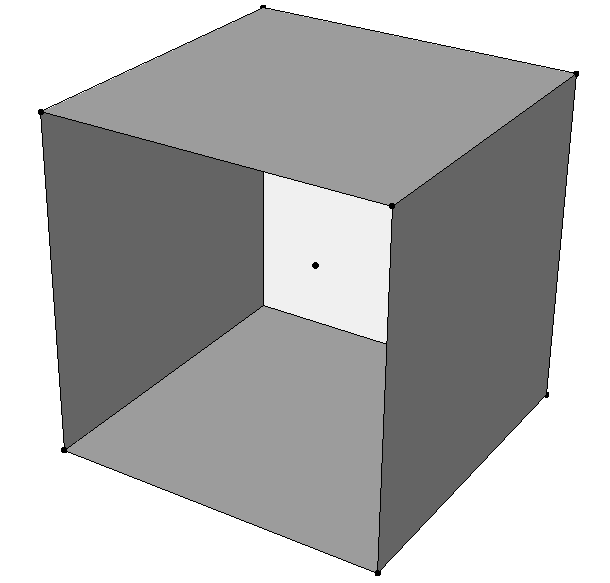
\includegraphics[width=8cm, height=8cm]{test3_smd}
  \caption{Cube with vertex placed at center. Front face hidden to 
        to show interior.}
  \label{fig:vert1model}
\end{figure}

\begin{figure}[H]
  \centering
  \subfigure[Exterior view.]
    { 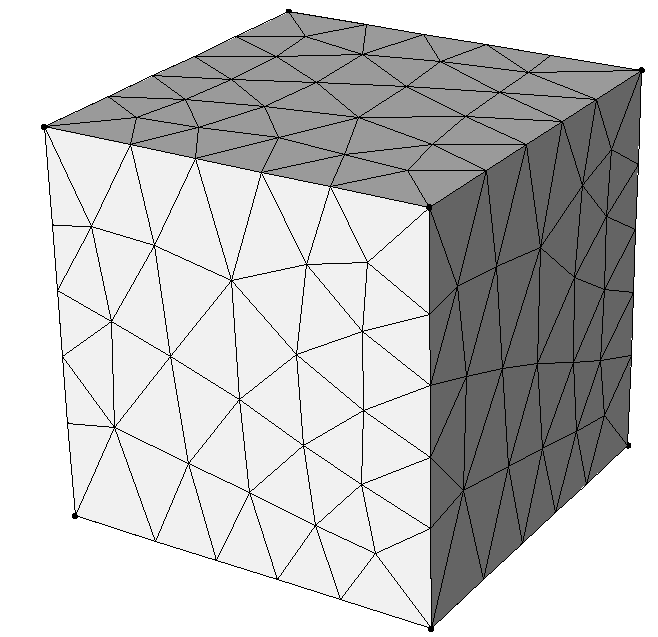
\includegraphics[width=0.45\textwidth, height=0.45\textwidth]{test3_sms}}
  \subfigure[Clipped view.]
    { 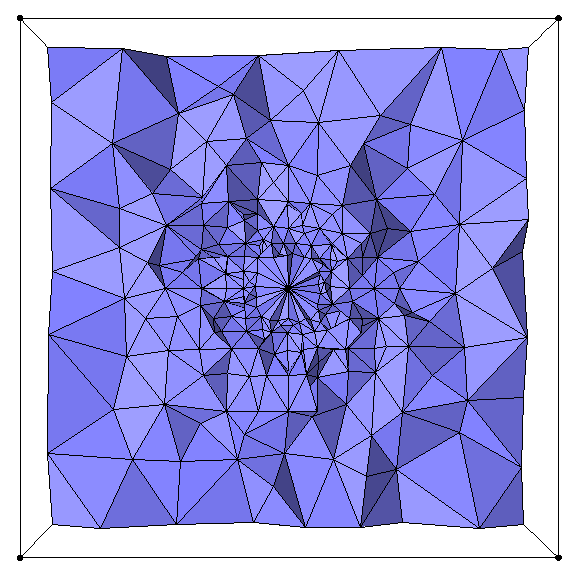
\includegraphics[width=0.45\textwidth, height=0.45\textwidth]{test3_sms_clipped}}
  \caption{Mesh of cube with vertex placed at center.}
  \label{fig:vert1mesh}
\end{figure}

The second case placed a vertex in the center of a face of a three dimensional 
model. The global mesh refinement level was set to 0.9 and the refinement
level of the vertex was set to 0.1. 
The resulting model is shown in Figure \ref{fig:vert2model}.
The resulting mesh is shown in Figure \ref{fig:vert2mesh}.

\begin{figure}[H]
  \centering
  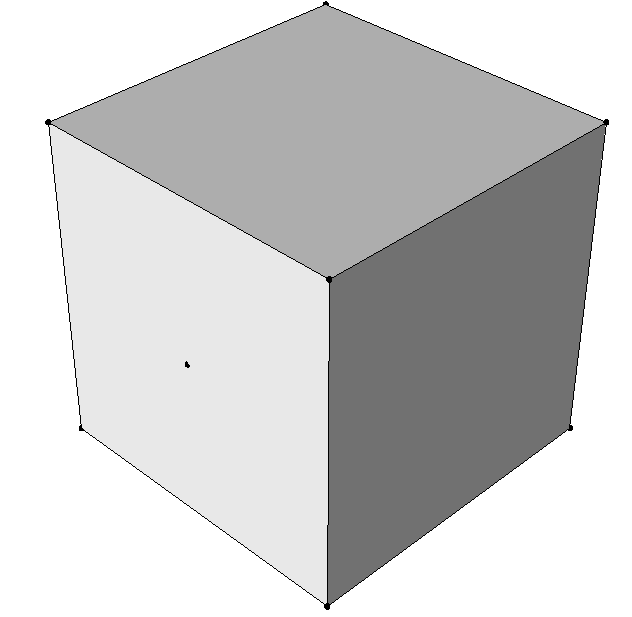
\includegraphics[width=8cm, height=8cm]{test4_smd}
  \caption{Cube with vertex placed at center of front face.}
  \label{fig:vert2model}
\end{figure}

\begin{figure}[H]
  \centering
  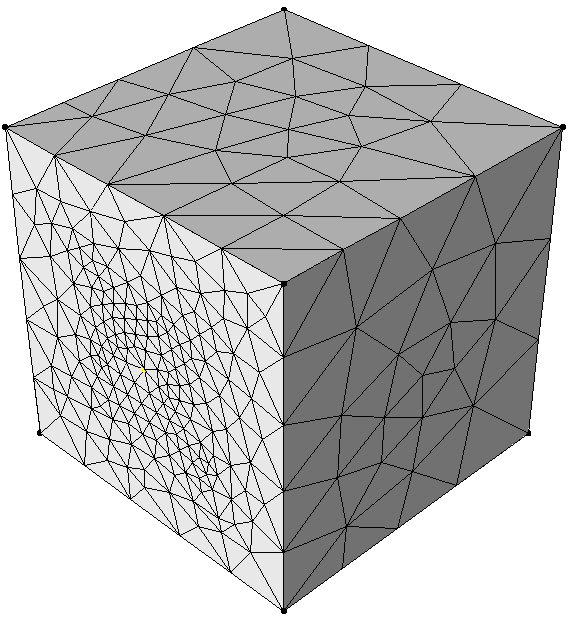
\includegraphics[width=8cm, height=8cm]{test4_sms}
  \caption{Mesh of cube with vertex on center of front face.}
  \label{fig:vert2mesh}
\end{figure}

The third case placed a vertex on a preexisting model edge. The global
mesh refinement level was 0.9 and the local refinement level for the
vertex was 0.1.
The resulting model is shown in Figure \ref{fig:vert3model}.
The resulting mesh is shown in Figure \ref{fig:vert3mesh}.

\begin{figure}[H]
  \centering
  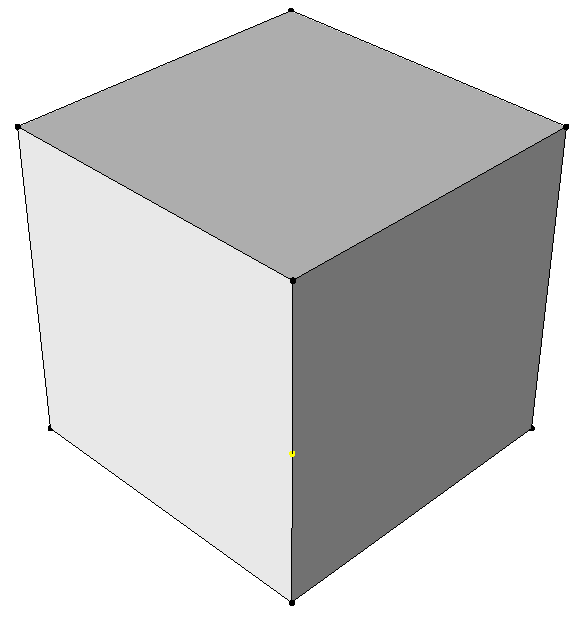
\includegraphics[width=8cm, height=8cm]{test5_smd}
  \caption{Cube with vertex placed at center of edge.}
  \label{fig:vert3model}
\end{figure}

\begin{figure}[H]
  \centering
  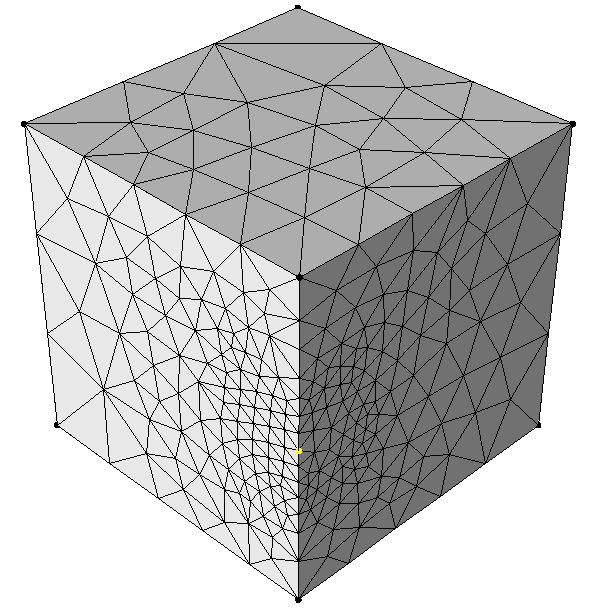
\includegraphics[width=8cm, height=8cm]{test5_sms}
  \caption{Mesh of cube with vertex on center of edge.}
  \label{fig:vert3mesh}
\end{figure}

As shown in Figures \ref{fig:vert1model} through \ref{fig:vert3mesh}, 
the gmd method \emph{place\_point()} is able to correctly determine 
the model classification given a user defined location. It is also 
able to change the local mesh refinement level to a user's specification. 

\subsection{Edge Placement} \label{subsec:edgeTest}
Edge placement was tested in four cases. Similar to the vertex tests 
presented in subsection \ref{subsec:vertexTest}, models and meshes
were created and written to disk; expected behavior and classification
was confirmed through both the Simmetrix APIs and the GUI.

The first test placed a fully interior edge inside a model region. 
The edge was created as a rational basis spline with five control points; 
each control point was inside the model region.
The global mesh refinement was set to 0.9 and the local set to 0.1. 
A wire frame view of the created model is shown in Figure \ref{fig:edge1model}.
A clipped view of the mesh is shown in Figure \ref{fig:edge1mesh}.

\begin{figure}[H]
  \centering
  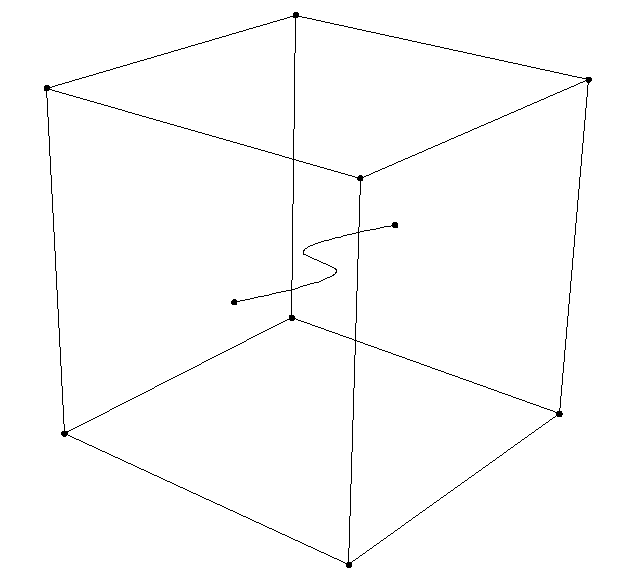
\includegraphics[width=8cm, height=8cm]{test6_smd}
  \caption{Cube with edge placed near center of region.}
  \label{fig:edge1model}
\end{figure}

\begin{figure}[H]
  \centering
  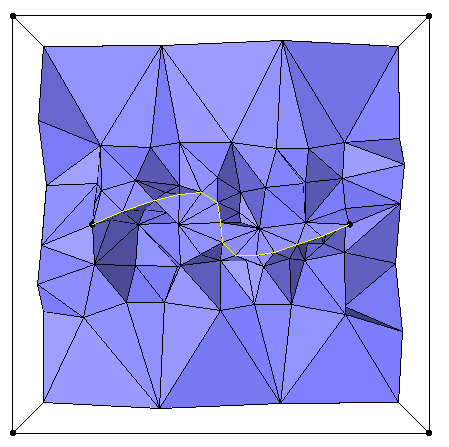
\includegraphics[width=8cm, height=8cm]{test6_sms_clipped}
  \caption{Clipped view of mesh for cube with edge near center of region. 
          The edge is highlighted in yellow.}
  \label{fig:edge1mesh}
\end{figure}

The second test placed an edge whose control points all laid on the same 
model face. 
The edge was created as a rational basis spline with five control points.
The global mesh refinement was set to 0.9 and the local set to 0.1. 
The created model is shown in Figure \ref{fig:edge2model}.
A view of the mesh is shown in Figure \ref{fig:edge2mesh}.

\begin{figure}[H]
  \centering
  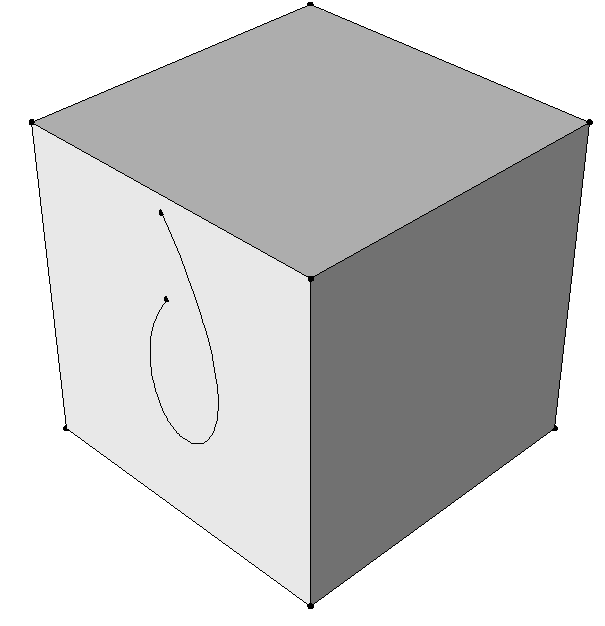
\includegraphics[width=8cm, height=8cm]{test7_smd}
  \caption{Cube with edge placed on model front face.}
  \label{fig:edge2model}
\end{figure}

\begin{figure}[H]
  \centering
  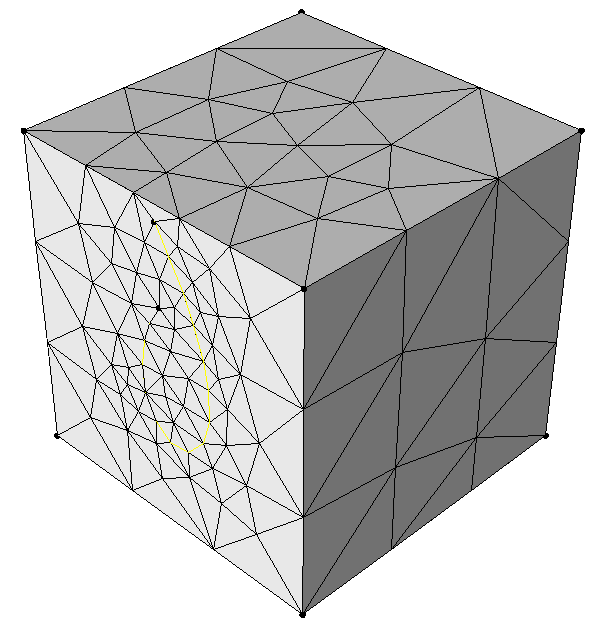
\includegraphics[width=8cm, height=8cm]{test7_sms}
  \caption{Clipped view of mesh for cube with edge on face. 
          The edge is highlighted in yellow.}
  \label{fig:edge2mesh}
\end{figure}

The third test placed an edge that started on a model face and 
terminated in the interior of the model region. 
The edge was created as a rational basis spline with five control points.
The global mesh refinement was set to 0.9 and the local set to 0.1. 
Two images of the created model are shown in Figure \ref{fig:edge3model}.
A external and clipped view of the mesh are shown in Figure \ref{fig:edge3mesh}.

\begin{figure}[H]
  \centering
  \subfigure[Solid view.]
    { 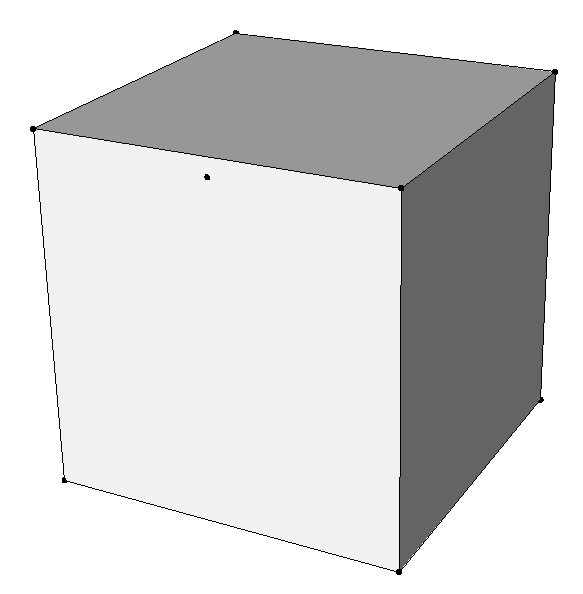
\includegraphics[width=0.45\textwidth, height=0.45\textwidth]{test8_smd}}
  \subfigure[Wire frame view.]
    { 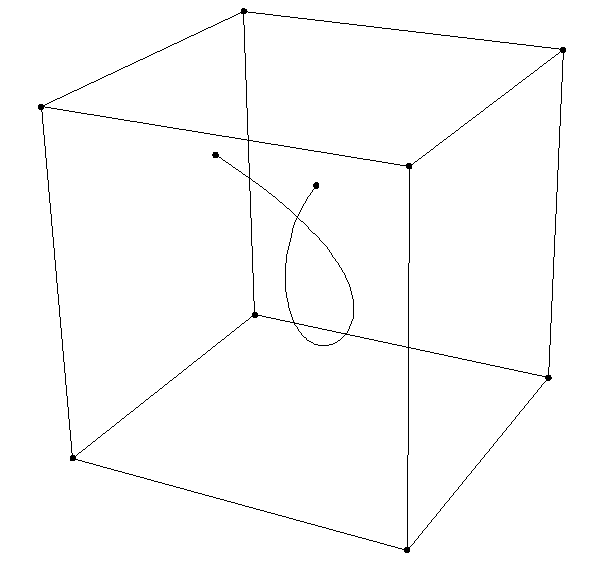
\includegraphics[width=0.45\textwidth, height=0.45\textwidth]{test8_smd_wire}}
  \caption{Model with edge inserted. Edge begins on front face and terminates 
        with in the model region.}
  \label{fig:edge3model}
\end{figure}

\begin{figure}[H]
  \centering
  \subfigure[External view.]
    { 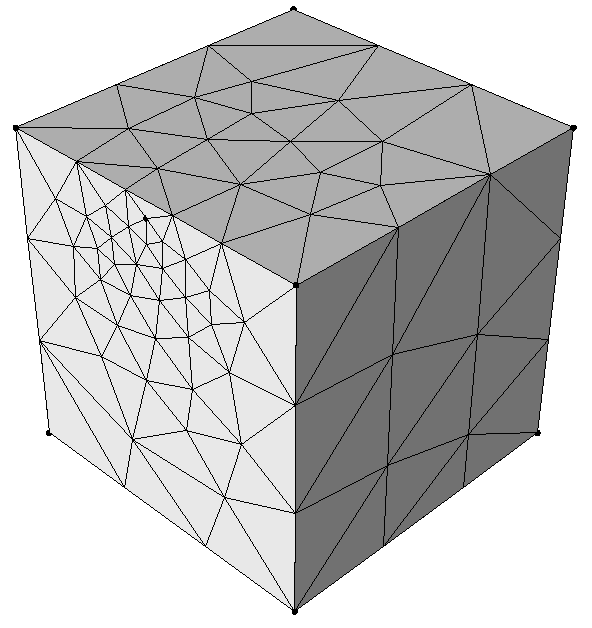
\includegraphics[width=0.45\textwidth, height=0.45\textwidth]{test8_sms}}
  \subfigure[Clipped view.]
    { 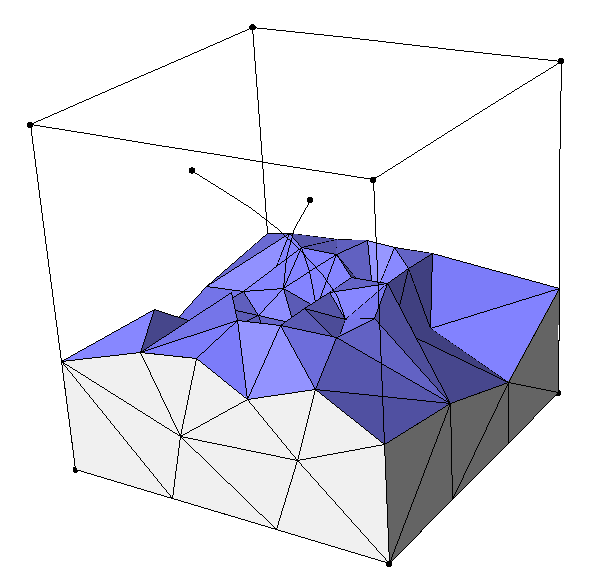
\includegraphics[width=0.45\textwidth, height=0.45\textwidth]{test8_sms_clipped}}
  \caption{Mesh of model with edge from face to region inserted.}
  \label{fig:edge3mesh}
\end{figure}

The fourth test placed an edge that started on a model edge and terminated 
with in the model region. 
The edge was created as a rational basis spline with five control points.
The global mesh refinement was set to 0.9 and the local set to 0.1. 
Two images of the created model are shown in Figure \ref{fig:edge4model}.
A external and clipped view of the mesh are shown in Figure \ref{fig:edge4mesh}.

\begin{figure}[H]
  \centering
  \subfigure[Solid view.]
    { 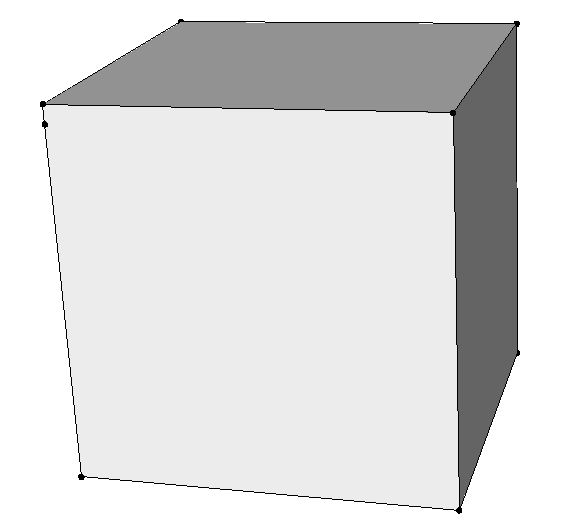
\includegraphics[width=0.45\textwidth, height=0.45\textwidth]{test9_smd}}
  \subfigure[Wire frame view.]
    { 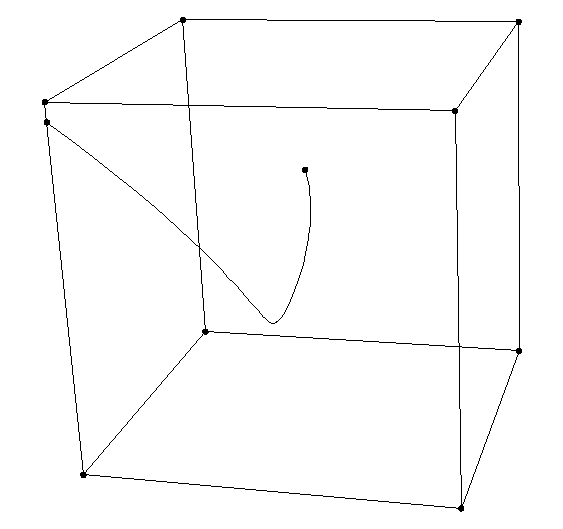
\includegraphics[width=0.45\textwidth, height=0.45\textwidth]{test9_smd_wire}}
  \caption{Model with edge inserted. Edge begins on left-most vertical model edge
        and terminates within the model region.}
  \label{fig:edge4model}
\end{figure}

\begin{figure}[H]
  \centering
  \subfigure[External view.]
    { 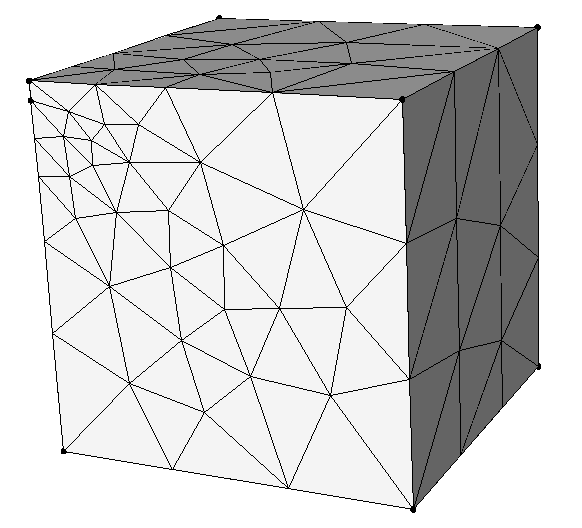
\includegraphics[width=0.45\textwidth, height=0.45\textwidth]{test9_sms}}
  \subfigure[Clipped view.]
    { 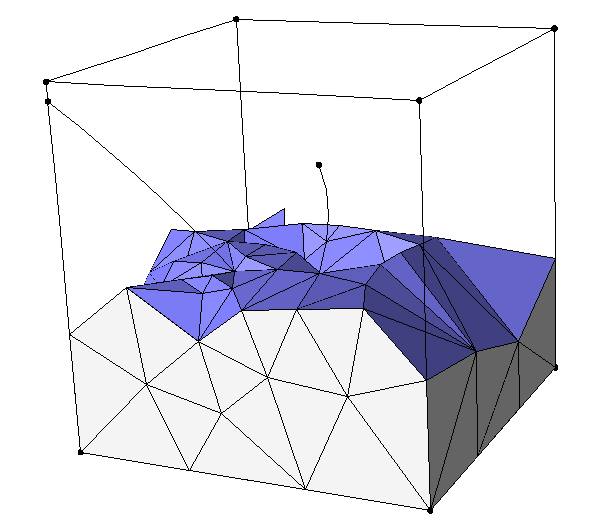
\includegraphics[width=0.45\textwidth, height=0.45\textwidth]{test9_sms_clipped}}
  \caption{Mesh of model with edge from edge to region inserted.}
  \label{fig:edge4mesh}
\end{figure}

As shown in Figures \ref{fig:edge1model} through \ref{fig:edge4mesh}, 
the gmd method \emph{place\_edge()} is able to correctly determine 
the model classification given user defined spline parameters. It is also 
able to change the local mesh refinement level to a user's specification. 

\subsection{Face Placement} \label{subsec:faceTest}
Face placement was tested similarly to both the vertex and edge
tests described in subsections \ref{subsec:vertexTest} and \ref{subsec:edgeTest}.
In total, three tests were performed. For each test, the created 
models and meshes were written to disk and viewed in the Simmetrix GUI.
Classifications of model entities were confirmed through both the GUI and 
APIs where applicable.

The first face placement test created a model face that was completely interior
to a model region.
The face, and its bounding edges,  were created as 
as a rational basis surface and splines. In total, 12 control points were 
defined; each control point was inside the model region and created a $4\times3$
grid. The global mesh refinement was set to 0.9 and the local set to 0.1. 
A face view of the created model is shown in Figure \ref{fig:face1model}.
The face and clipped view of the mesh are shown in Figure \ref{fig:face1mesh}.

\begin{figure}[H]
  \centering
  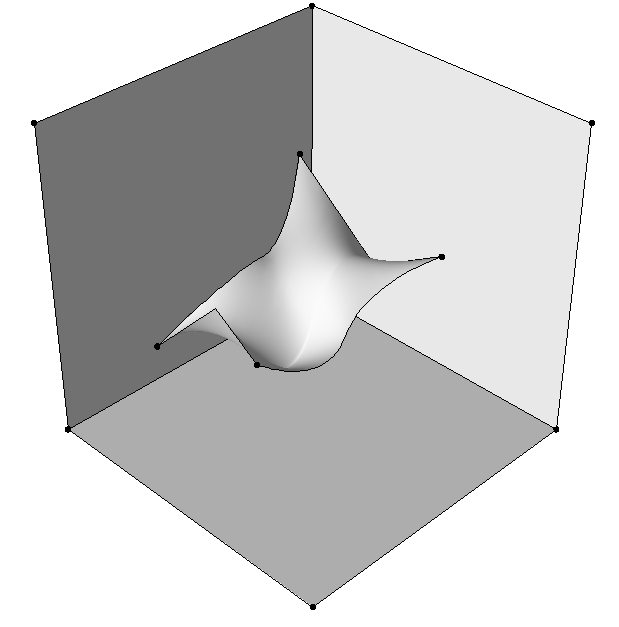
\includegraphics[width=8cm, height=8cm]{test10_smd_seeThrough}
  \caption{Cube with face created within the model region. Forward three face
        were made transparent to show in the internal face.}
  \label{fig:face1model}
\end{figure}

\begin{figure}[H]
  \centering
  \subfigure[Face view.]
    { 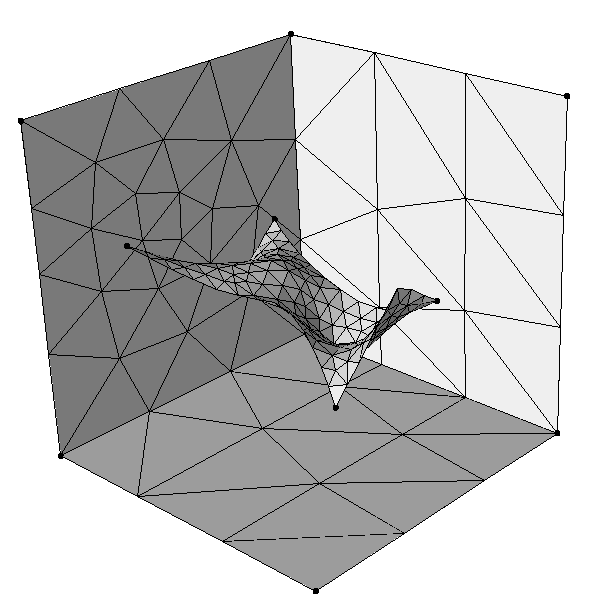
\includegraphics[width=0.45\textwidth, height=0.45\textwidth]{test10_sms_seeThrough}}
  \subfigure[Clipped view.]
    { 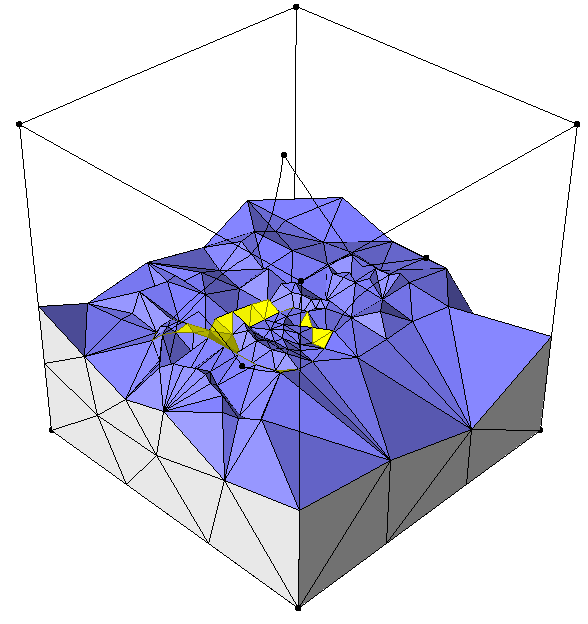
\includegraphics[width=0.45\textwidth, height=0.45\textwidth]{test10_sms_clipped}}
  \caption{Mesh of model with interior face.
        Yellow mesh element faces indicate the mesh face is coplanar with the
        model face. Note the view is rotated right by $90^{\circ}$ with respect 
        to Figure \ref{fig:face1model}.}
  \label{fig:face1mesh}
\end{figure}

The second face placement test created a model face that was completely 
interior to a model region except for one corner vertex. 
The face, and its bounding edges,  were created as 
as a rational basis surface and splines. In total, 12 control points were 
defined; all but one control point was inside the model region and created a $4\times3$
grid. The global mesh refinement was set to 0.9 and the local set to 0.1. 
A front and face view of the created model are shown in Figure \ref{fig:face2model}.
The face and clipped view of the mesh are shown in Figure \ref{fig:face2mesh}.
An external view of the mesh is shown in Appendix \ref{subsec:test11Img}.

\begin{figure}[H]
  \centering
  \subfigure[Solid view.]
    { 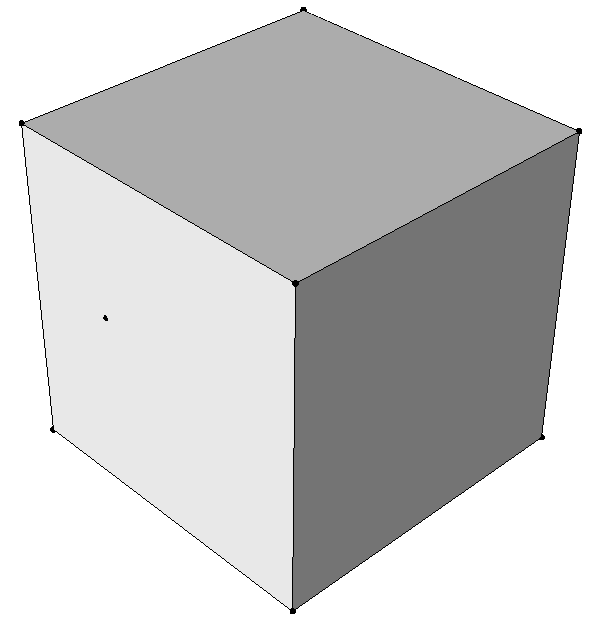
\includegraphics[width=0.45\textwidth, height=0.45\textwidth]{test11_smd}}
  \subfigure[Face view.]
    { 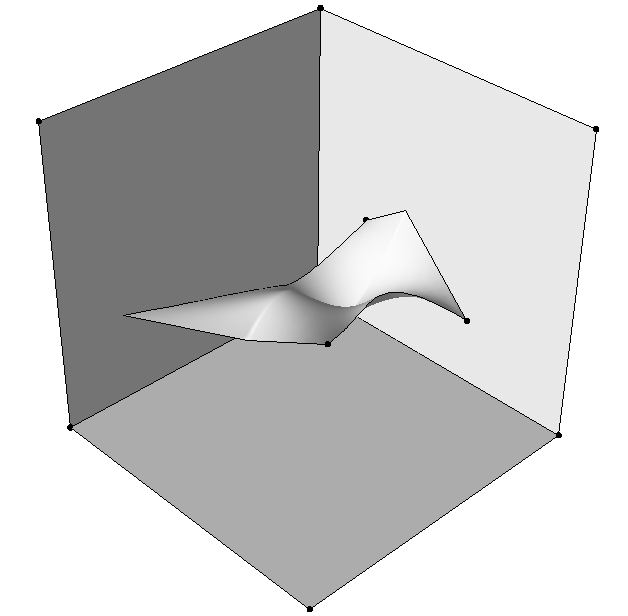
\includegraphics[width=0.45\textwidth, height=0.45\textwidth]{test11_smd_seeThrough}}
  \caption{Model with face inserted. Face is fully interior except for one point.
        The point is shown on the leftmost face in (a).}
  \label{fig:face2model}
\end{figure}

\begin{figure}[H]
  \centering
  \subfigure[Face view.]
    { 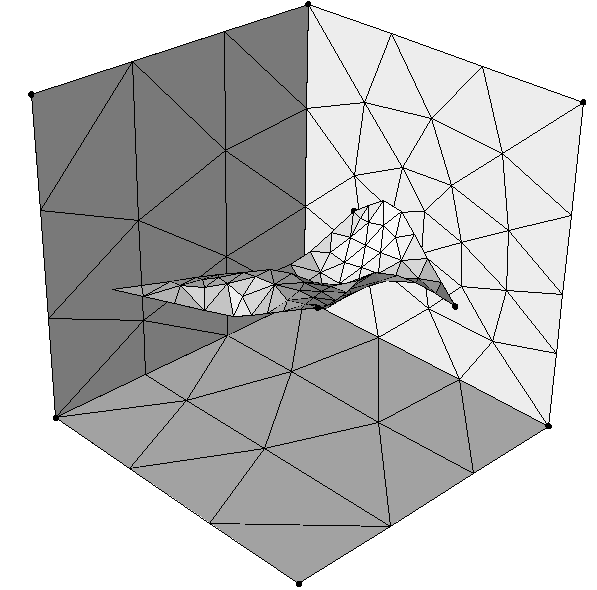
\includegraphics[width=0.45\textwidth, height=0.45\textwidth]{test11_sms_seeThrough}}
  \subfigure[Clipped view.]
    { 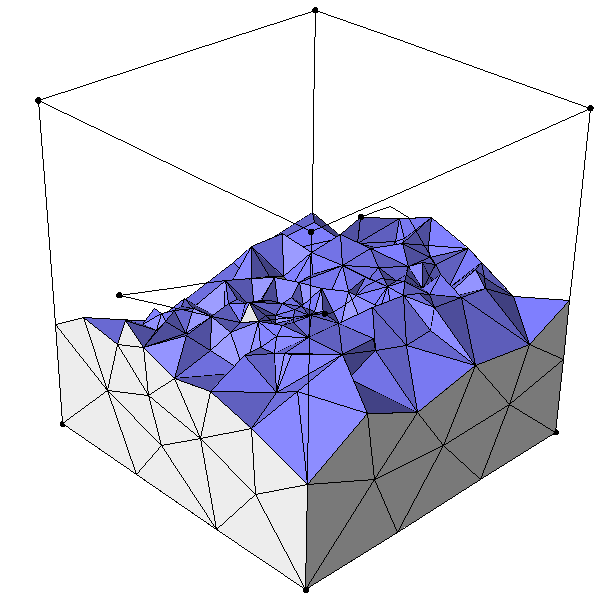
\includegraphics[width=0.45\textwidth, height=0.45\textwidth]{test11_sms_clipped}}
  \caption{Mesh of model with interior face except for one point.}
  \label{fig:face2mesh}
\end{figure}

The third face placement test created a model face that was completely 
interior to a model region except for one edge.
The face, and its bounding edges,  were created as 
as a rational basis surface and splines. In total, 12 control points were 
defined; the control points created a $4\times3$
grid. The global mesh refinement was set to 0.9 and the local set to 0.1. 
A front and face view of the created model are shown in Figure \ref{fig:face3model}.
The face and clipped view of the mesh are shown in Figure \ref{fig:face3mesh}.
An external view of the mesh is shown in Appendix \ref{subsec:test12Img}.

\begin{figure}[H]
  \centering
  \subfigure[Solid view.]
    { 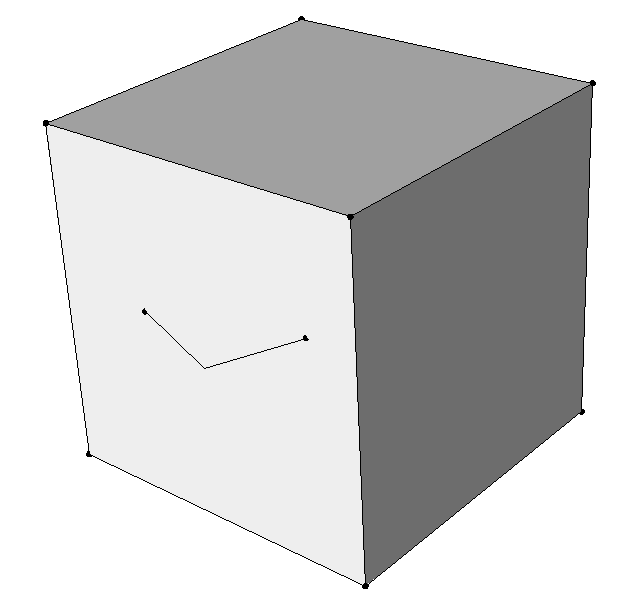
\includegraphics[width=0.45\textwidth, height=0.45\textwidth]{test12_smd}}
  \subfigure[Face view.]
    { 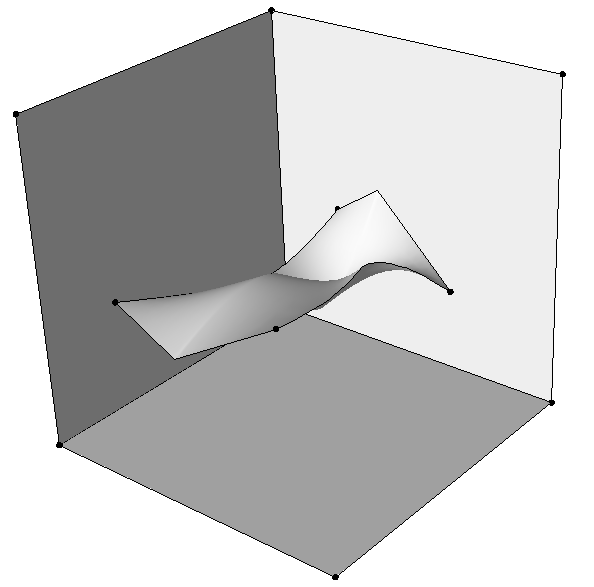
\includegraphics[width=0.45\textwidth, height=0.45\textwidth]{test12_smd_seeThrough}}
  \caption{Model with face inserted. Face is fully interior except for one edge.
        The edge is shown on the leftmost face in (a).}
  \label{fig:face3model}
\end{figure}

\begin{figure}[H]
  \centering
  \subfigure[Face view.]
    { 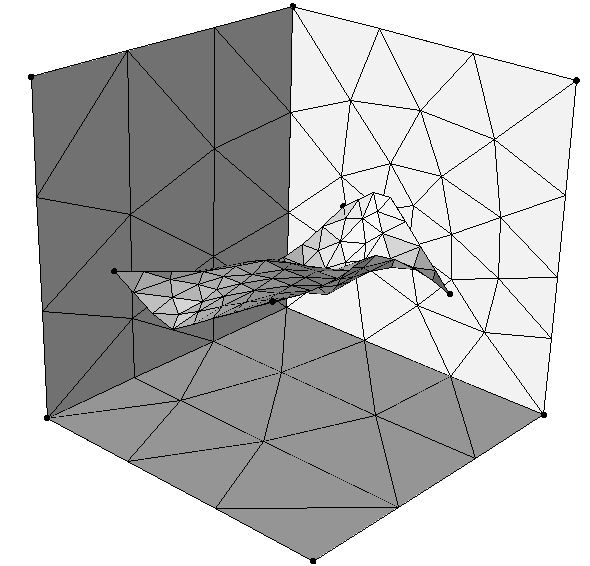
\includegraphics[width=0.45\textwidth, height=0.45\textwidth]{test12_sms_seeThrough}}
  \subfigure[Clipped view.]
    { 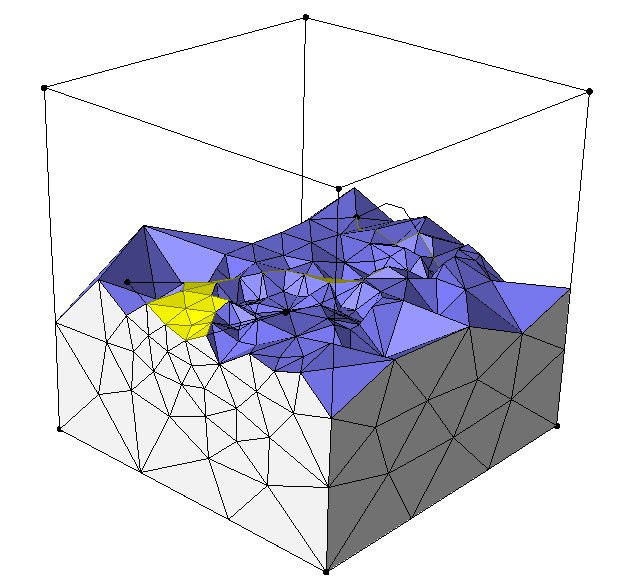
\includegraphics[width=0.45\textwidth, height=0.45\textwidth]{test12_sms_clipped}}
  \caption{Mesh of model with interior face except for one edge. 
        Yellow mesh element faces indicate the mesh face is coplanar with the
        model face.}
  \label{fig:face3mesh}
\end{figure}

As shown in Figures \ref{fig:face1model} through \ref{fig:face3mesh}, 
the gmd method \emph{place\_face()} is able to correctly determine 
the model classification given user defined surface parameters. It is also 
able to change the local mesh refinement level to a user's specification. 

\section{Conclusion} \label{sec:conclusion}
The purpose of this project was to create an interface to the 
Simmetrix APIs that allows for model and mesh modification. This
was to include placement of vertices, edges, and surfaces. The 
interface was to be general enough to allow for the edges not be limited
to straight lines and the surfaces not to be limited to flat planes. 
Additionally, the modified model was to remain topologically valid
to allow for proper discretization and interrogation. 

These features were completed in the project.
Vertex placement is described in subsection \ref{subsec:vertex}
and is demonstrated in three examples in subsection \ref{subsec:vertexTest}.
Edge placement is described in subsection \ref{subsec:edge}
and is demonstrated in four examples in subsection \ref{subsec:edgeTest}.
Face placement is described in subsection \ref{subsec:face}
and is demonstrated in three examples in subsection \ref{subsec:faceTest}.
The topology of the lower order entities is also valid since 
higher order geometric features make use of lower order ones.
For example, if the method which placed vertices did not reliably create
topologically valid vertices, then neither the \emph{place\_edge()} or 
\emph{place\_face()} would work properly. 

\subsection{Future Work} \label{subsec:future}
A possible improvement to the created code is to allow for parallel 
model modification or model discretization. Currently, only one
data structure that represents the model exists at any given time. 
This then leads to one data structure that represents the mesh. 
A parallel representation could use one common base model 
with different modification happening on different processors. 
Another possibility is to have a parallel mesh generated 
instead of a serial one.

The code currently can only handle native and non-manifold models, 
not assembly models. Additional work could be done to allow
for modification of theses types of models. This would mostly
include changes to region and part based functions. These changes 
include accounting for multiple parts and regions along with 
their interactions.

Work can be done that would allow for geometric entity deletion
that preserves topological validity. For example, a user can 
currently delete any edge. This will yield a topologically 
invalid model if the edge was one of the bounding edge of a 
model face. This addition of features could also
include methods to trim or extend model entities as well. 

\newpage
\begin{thebibliography}{99}

\bibitem{weiler86}
Weiler, Kevin J.
(1986).
Topological Structures for Geometric Modeling.
(Doctoral dissertation).

\bibitem{zhangThesis}
Zhang, Lijuan.
(2013).
Microstructural modeling of cross-linked fiber network embedded in continuous matrix.
(Doctoral dissertation).

\bibitem{askeland}
Askeland, Donald R., Fulay, Pradeep P., Wright, Wendelin J.
(2011).
The Science and Engineering of Materials.
Sixth ed.
Stamford, CT: Cengage Learning.
Print.

\bibitem{Simmetrix}
Simmetrix Inc., 
"The simulation modeling suite."
\textit{[Online]. Available: http://www.simmetrix.com/.}

\end{thebibliography}

\newpage
\appendix
\section{Code} \label{sec:code}

\subsection{main.cpp} \label{subsec:main_cpp}
\lstinputlisting{/lore/clougj/GeoMod/src/main.cpp}

\subsection{GeoMod\_Tests.hpp} \label{subsec:Tests_hpp}
\lstinputlisting{/lore/clougj/GeoMod/src/GeoMod_Tests.hpp}
\subsection{GeoMod\_Tests.cpp} \label{subsec:Tests_cpp}
\lstinputlisting{/lore/clougj/GeoMod/src/GeoMod_Tests.cpp}

\subsection{GeoMod\_gmd.hpp} \label{subsec:gmd_hpp}
\lstinputlisting{/lore/clougj/GeoMod/src/GeoMod_gmd_t.hpp}
\subsection{GeoMod\_gmd.cpp} \label{subsec:gmd_cpp}
\lstinputlisting{/lore/clougj/GeoMod/src/GeoMod_gmd_t.cpp}

\subsection{GeoMod\_model\_helper.hpp} \label{subsec:model_hpp}
\lstinputlisting{/lore/clougj/GeoMod/src/GeoMod_model_helper.hpp}
\subsection{GeoMod\_model\_helper.cpp} \label{subsec:model_cpp}
\lstinputlisting{/lore/clougj/GeoMod/src/GeoMod_model_helper.cpp}

\subsection{GeoMod\_mesh\_helper.hpp} \label{subsec:mesh_hpp}
\lstinputlisting{/lore/clougj/GeoMod/src/GeoMod_mesh_helper.hpp}
\subsection{GeoMod\_mesh\_helper.cpp} \label{subsec:mesh_cpp}
\lstinputlisting{/lore/clougj/GeoMod/src/GeoMod_mesh_helper.cpp}

\subsection{GeoMod\_printer.hpp} \label{subsec:printer_hpp}
\lstinputlisting{/lore/clougj/GeoMod/src/GeoMod_printer.hpp}
\subsection{GeoMod\_printer.cpp} \label{subsec:printer_cpp}
\lstinputlisting{/lore/clougj/GeoMod/src/GeoMod_printer.cpp}

\subsection{GeoMod\_coords.hpp} \label{subsec:coords_hpp}
\lstinputlisting{/lore/clougj/GeoMod/src/GeoMod_coords.hpp}
\subsection{GeoMod\_coords.cpp} \label{subsec:coords_cpp}
\lstinputlisting{/lore/clougj/GeoMod/src/GeoMod_coords.cpp}

\subsection{GeoMod\_util.hpp} \label{subsec:util_hpp}
\lstinputlisting{/lore/clougj/GeoMod/src/GeoMod_util.hpp}
\subsection{GeoMod\_util.cpp} \label{subsec:util_cpp}
\lstinputlisting{/lore/clougj/GeoMod/src/GeoMod_util.cpp}

\subsection{GeoMod\_SIM.hpp} \label{subsec:SIM_hpp}
\lstinputlisting{/lore/clougj/GeoMod/src/GeoMod_SIM.hpp}

\newpage
\section{Supplementary Images} \label{sec:img}
\subsection{Model and Mesh of Test 1} \label{subsec:test1Img}
\begin{figure}[H]
  \centering
  \subfigure
    { 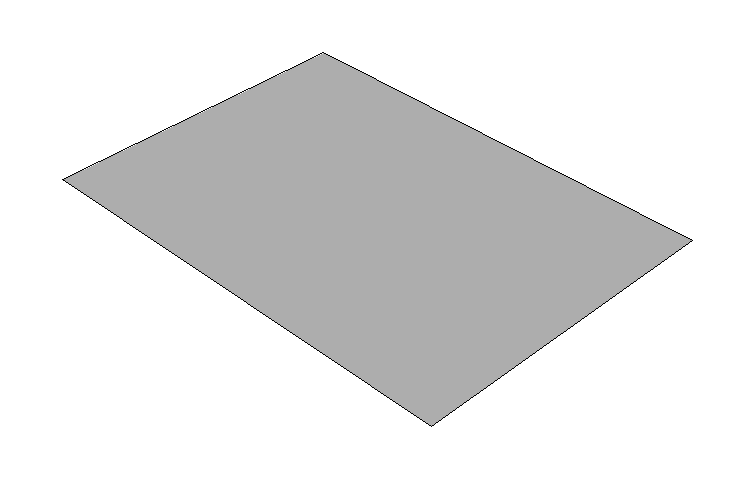
\includegraphics[width=0.45\textwidth, height=0.45\textwidth]{test1_smd}}
  \subfigure
    { 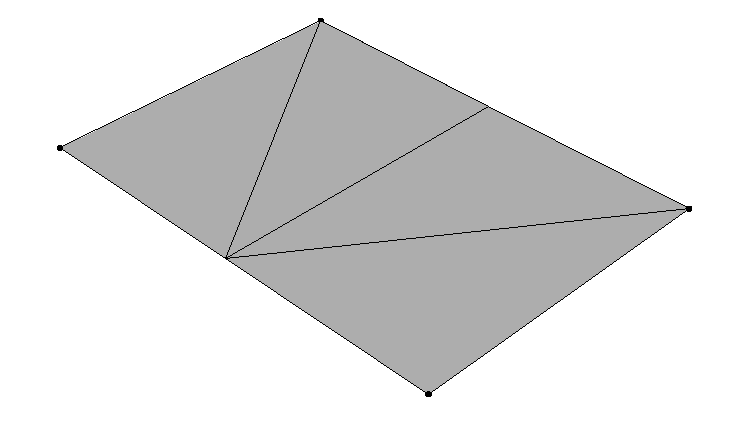
\includegraphics[width=0.45\textwidth, height=0.45\textwidth]{test1_sms}}
\end{figure}

\subsection{Model and Mesh of Test 2} \label{subsec:test2Img}
\begin{figure}[H]
  \centering
  \subfigure
    { 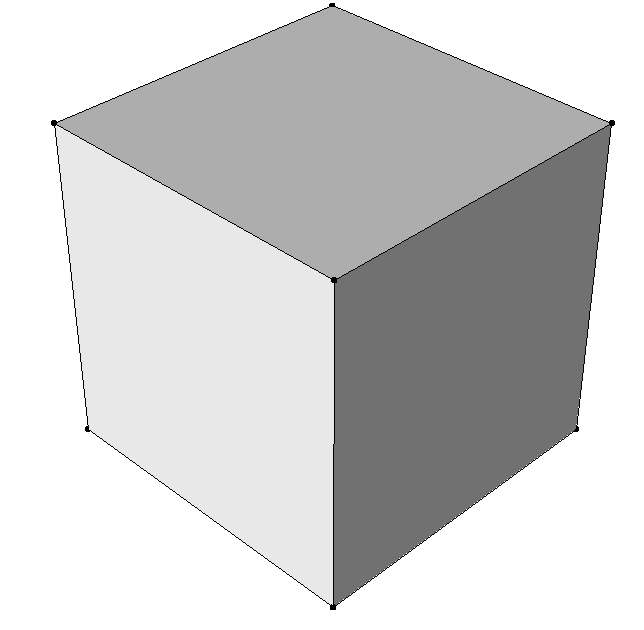
\includegraphics[width=0.45\textwidth, height=0.45\textwidth]{test2_smd}}
  \subfigure
    { 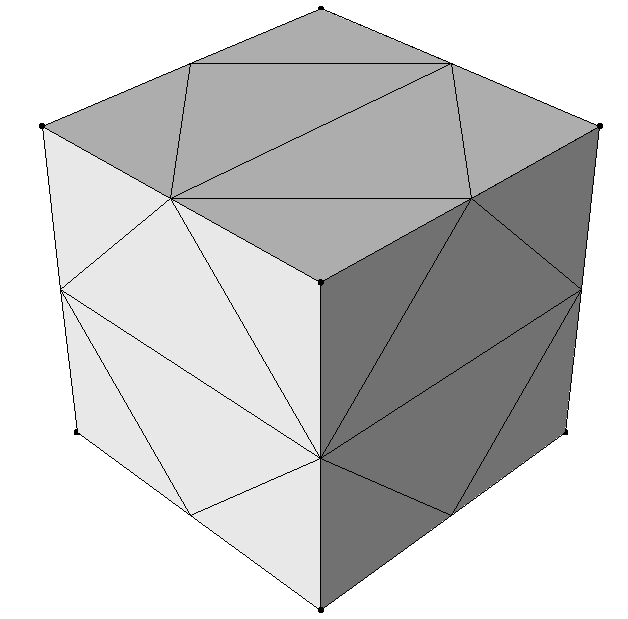
\includegraphics[width=0.45\textwidth, height=0.45\textwidth]{test2_sms}}
\end{figure}

\subsection{Mesh of Test 11} \label{subsec:test11Img}
\begin{figure}[H]
  \centering
  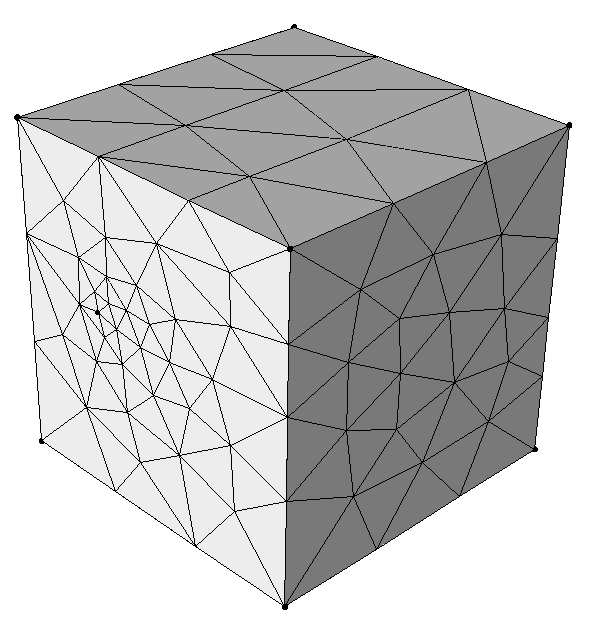
\includegraphics[width=8cm, height=8cm]{test11_sms}
\end{figure}

\subsection{Mesh of Test 12} \label{subsec:test12Img}
\begin{figure}[H]
  \centering
  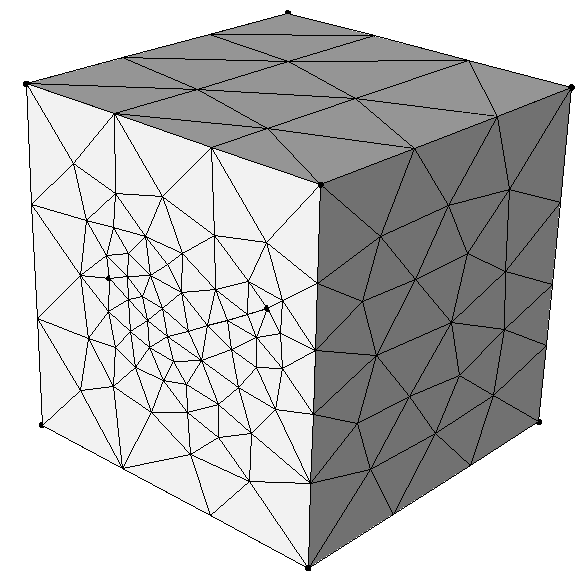
\includegraphics[width=8cm, height=8cm]{test12_sms}
\end{figure}

\end{document}
